\section{A historical context of diffraction theory: from shadows to the vector world}

	For more than two thousand years, from Euclid to the threshold of the Renaissance,
	geometrical optics rested on a single, almost self-evident assumption: light travels in
	straight lines \cite{herzberger1966optics}. A straight ray casts a straight-edged shadow,
	and every child who has ever played with their own silhouette on a wall has confirmed it
	a thousand times. This picture explained mirrors, lenses and eclipses so well that for
	centuries nobody thought to look closely at the edge of a shadow itself - to ask what
	really happens in that thin borderland where light stops and darkness begins. Diffraction
	is the story of what was hiding in that borderland, and of how a single overlooked detail,
	pursued patiently over three centuries, forced physicists to rebuild their entire
	understanding of what light is. It is, in a real sense, the story of light refusing to be
	simplified.

	The first person to look carefully enough was an Italian Jesuit named Francesco Maria
	Grimaldi. Sometime around 1660, working in a darkened room in Bologna, Grimaldi let a
	narrow beam of sunlight fall through a tiny aperture and cross the edge of a rod before
	striking a screen. Ordinary geometry made a firm prediction: a sharp-edged shadow, dark on
	one side and bright on the other, with nothing more to say. What Grimaldi saw instead was
	stranger and far more delicate - the boundary of the shadow was not a clean line but a
	soft fringe, laced with faint bands of colour, and the shadow itself was slightly wider
	than pure geometry allowed. Light was somehow reaching into the space it was not supposed
	to reach, and bending in ways no ray could bend. Grimaldi did not live to see his work in
	print; his observations appeared only after his death, in the 1665 book
	\textit{Physico-Mathesis de Lumine} \cite{grimaldi1665physico}. There he gave the effect
	its name, \textit{diffractio}, from the Latin for ``breaking into pieces,'' because it
	looked to him as though the light itself had been shattered at the edge of the obstacle.
	It was a remarkably prescient observation, made with nothing more than sunlight, a dark
	room and a sharp eye - and for a long time, almost nobody noticed it had been made.

	The reason nobody noticed is largely one man's name: Isaac Newton. Newton himself had
	seen delicate coloured rings form between a lens and a flat glass plate - the pattern we
	still call Newton's rings today - and he described them meticulously in his own
	\textit{Opticks} of 1704 \cite{newton1704opticks}. Yet Newton remained convinced that
	light was made of small particles, corpuscles, shot out in straight lines, and he folded
	these puzzling colours into that picture as best he could rather than let them overturn
	it. Newton's scientific authority in the eighteenth century was so enormous that to argue
	against him was close to professional suicide, and so Grimaldi's fringes, and the
	wave-like reasoning that might have explained them, were quietly set aside for more than a
	hundred years. It is one of the great cautionary tales of physics: the evidence for
	diffraction was sitting in plain sight the entire time, waiting for someone willing to
	take it seriously.

	Someone did, although his idea arrived slightly ahead of its time and without quite
	enough machinery to finish the job. In 1690 the Dutch physicist Christiaan Huygens
	proposed, in his \textit{Traité de la Lumière} \cite{huygens1690traite}, an almost
	playful way of picturing how a wave moves forward. Imagine, Huygens said, that every
	single point on a wavefront is itself a tiny source, spraying out its own small circular
	ripple. A moment later, the new wavefront is simply the smooth envelope that wraps around
	all of those countless little ripples at once. This picture - now known as
	Huygens's principle - explained reflection and refraction beautifully, and it hinted that
	a wave could indeed sneak sideways into a geometrical shadow, since the ripples spreading
	from points near the edge of an obstacle have nowhere to go but into that forbidden space.
	What Huygens's construction could not yet explain was why the resulting light and dark
	fringes appeared exactly where they did, because he had no notion that the little ripples
	might reinforce each other in some places and cancel each other in others. That missing
	idea was interference, and supplying it would take more than a century.

	It finally arrived in a remarkable few years at the start of the nineteenth century. In
	1801, the English polymath Thomas Young performed the experiment that every optics
	student meets sooner or later: he let light pass through two narrow, closely spaced slits
	and watched the pattern it formed on a screen beyond \cite{young1804bakerian}. Instead of
	two bright bands, he saw many - an entire sequence of bright and dark stripes, exactly as
	one would expect if two overlapping ripples on a pond could sometimes crest together and
	sometimes cancel to stillness. Light, Young concluded, must be a wave, and waves can add
	or subtract. It was a devastatingly simple experiment carrying an enormous conclusion, and
	for exactly that reason it was met in England with scorn rather than applause; attacking
	Newton was still not a popular sport. Vindication came from France. Between 1815 and 1820
	the young engineer Augustin-Jean Fresnel took Huygens's wavelets and Young's interference
	and welded them into a single, quantitative principle - the Huygens-Fresnel principle -
	capable of predicting, for the first time, exactly how bright or dark any point in a
	diffraction pattern should be \cite{fresnel1819memoire}. Fresnel did not merely describe
	diffraction qualitatively, as Grimaldi and Huygens had; he calculated it, treating every
	point of an opening as a genuine source of secondary waves whose ripples had to be added
	together, crest against crest and trough against trough, to find the light at any point
	beyond.

	Fresnel's theory then delivered one of the most celebrated moments in the history of
	physics. The French Academy of Sciences, still largely unconvinced, set diffraction as
	the subject of a prize competition, and the mathematician Siméon Denis Poisson, a
	confirmed sceptic of the wave picture, examined Fresnel's equations looking for an
	absurdity that would sink them for good. He found what he was looking for, or thought he
	had: Fresnel's own mathematics predicted that at the very centre of the shadow cast by a
	small circular disc, directly behind the obstacle where common sense guarantees total
	darkness, there should be a bright spot of light. Poisson presented this as a
	reductio ad absurdum, confident that no such thing could ever be observed. The academy's
	chairman, Dominique Arago, decided to actually perform the experiment rather than argue
	about it - and there, glowing faintly at the heart of the disc's shadow, was the spot
	Poisson had predicted in mockery. The Poisson-Arago spot, as it is now known with a
	certain irony, became one of the most dramatic experimental confirmations any theory has
	ever received, and it settled the contest between particles and waves for the rest of the
	century.

	Fresnel's success, however, was built on inspired intuition rather than rigorous
	derivation - his integral worked extremely well, but nobody had shown that it followed
	necessarily from the wave equation itself. That gap was closed in 1883 by the German
	physicist Gustav Kirchhoff, who used the mathematics of Green's theorem to derive
	Fresnel's diffraction integral directly from the wave equation, placing the whole
	construction on a firm mathematical foundation \cite{kirchhoff1883theorie}. Kirchhoff's
	formulation became, and largely remains, the working horse of what we now call the scalar
	theory of diffraction: it treats light as a single scalar ripple rather than a full
	electromagnetic vector, an approximation that works remarkably well whenever the
	obstacles involved are much larger than the wavelength of light. There was, admittedly, a
	subtle logical wrinkle in Kirchhoff's argument - his boundary conditions demanded that
	both the field and its derivative vanish simultaneously behind an opaque screen, a
	requirement that is mathematically over-strict - and it was Henri Poincaré who first
	pointed this out. The wrinkle was ironed out in 1896 by Arnold Sommerfeld, who found an
	alternative, fully self-consistent solution for diffraction by a straight edge and a
	half-plane, removing the inconsistency without sacrificing any of Kirchhoff's practical
	success \cite{sommerfeld1896mathematische, sommerfeld1954optics}.

	All of this, ingenious as it was, still treated light as a single wiggling number instead
	of the vector quantity that Maxwell's equations say it truly is - and by the early
	twentieth century that omission started to matter. In 1908 Gustav Mie solved Maxwell's
	equations exactly for light scattering off a small sphere, keeping the full vector and
	polarisation content of the field \cite{mie1908beitrage}; his result explains, among many
	other things, why the sky is blue and why clouds and milk are white, and it remains
	indispensable wherever light interacts with particles comparable in size to its own
	wavelength. The following year Peter Debye extended the same vector thinking to the tight
	focus of a lens, showing that near a sharp focal point the scalar approximation simply
	breaks down. The synthesis of everything that had come before - Fresnel's integral,
	Kirchhoff and Sommerfeld's rigour, and the full vector corrections of Mie and Debye - was
	finally gathered into a single, monumental reference by Max Born and Emil Wolf, whose
	\textit{Principles of Optics} (1959) has served as the field's bible ever since
	\cite{born1999principles}. Born and Wolf made explicit exactly when the simpler scalar
	picture is trustworthy and when it fails outright: in lenses of high numerical aperture,
	in anisotropic or chiral materials, and whenever the relevant structures shrink down to
	the scale of the wavelength itself, the vector nature of light can no longer be ignored.

	The invention of the laser in 1960 gave diffraction theory an entirely new practical
	urgency, since it suddenly supplied a light source coherent and controllable enough to
	exploit diffraction on purpose rather than merely tolerate it. Joseph Goodman's
	\textit{Introduction to Fourier Optics} (1968) reframed the whole subject in a beautifully
	economical way: an optical system, Goodman showed, can be treated as a kind of signal
	processor, and the diffraction pattern produced far from an aperture is, for all practical
	purposes, the same mathematical object as the Fourier transform of that aperture's shape
	\cite{goodman2005introduction}. This single reframing opened the door to holography, to
	diffractive lenses that focus light using etched patterns instead of curved glass, and to
	the computational correction of aberrations in modern cameras and telescopes.

	The story is very much still being written. Today, engineers etch \textbf{metasurfaces} -
	arrays of nanoscale structures far smaller than the wavelength of light - that reshape a
	wavefront's phase and polarisation point by point, allowing a sheet barely thicker than a
	human hair to do the work of a stack of lenses \cite{yu2011light}. Electron and X-ray
	diffraction, governed by exactly the same wave logic that Fresnel and Kirchhoff worked
	out for visible light, let scientists map the atomic architecture of crystals and
	molecules - it was X-ray diffraction, after all, that first revealed the double-helix
	structure of DNA. And diffraction sets an absolute, unbreakable limit on what any optical
	instrument can ever resolve: no telescope, however perfectly polished, and no microscope,
	however expensively built, can focus light down to a mathematical point, because the very
	act of passing light through a finite aperture spreads it out again. Every image a
	telescope or a microscope has ever produced, from the first blurred moons Galileo sketched
	to the sharpest pictures the largest observatories can deliver today, is diffraction's
	signature stamped on the light itself. Three and a half centuries after a Jesuit noticed
	that a shadow in a dark Bolognese room was not quite as sharp as geometry demanded,
	diffraction has grown from a curious imperfection into one of the deepest and most useful
	ideas in all of physics - and, as the chapters that follow will show in careful detail, it
	still has a great deal to teach us about the nature of light.

\section{Scalar theory of diffraction}\label{Sec:Diffraction}

	Electromagnetic waves are inherently vectorial: at each point $\vec{r}$ the electric
	field may exhibit a different state of polarisation. This property is expressed
	mathematically as

	\begin{equation}
	\vec{E}(\vec{r},t) = E(\vec{r},t) \, \hat{\vec{e}}(\vec{r},t),
	\end{equation}

	where $E(\vec{r},t)$ denotes the amplitude of the field and $\hat{\vec{e}}(\vec{r},t)$
	represents the polarisation vector, which besides varying in space may evolve in time in
	a stochastic manner.

	The associated wave equation then takes the form

	\begin{equation}
	\nabla^2 \left[ E(\vec{r},t)\hat{\vec{e}}(\vec{r},t) \right] - \mu\varepsilon \frac{\partial^2}{\partial t^2} \left[ E(\vec{r},t)\hat{\vec{e}}(\vec{r},t) \right] = 0,
	\end{equation}

	whose direct solution presents notable complexities. To tackle this problem one resorts
	to simplifying strategies, such as decomposing the field into scalar components. These
	scalar solutions may afterwards be combined to reconstruct the full vector behaviour.

	The temporal variation of amplitude, phase and polarisation is analysed rigorously
	through coherence theory (a topic explored in depth in Chapter~\ref{chap:Coherence}).
	Nevertheless, under certain approximations the temporal dependence of the amplitude is
	attributed solely to the intrinsic oscillations of the field, while the polarisation is
	regarded as static. The electric field then simplifies to

	\begin{equation}
	\vec{E}(\vec{r},t) = E(\vec{r},t) \, \hat{\vec{e}}(\vec{r}),
	\end{equation}

	allowing its expansion in an orthogonal polarisation basis,

	\begin{equation}
	\vec{E}(\vec{r},t) = E_1(\vec{r},t)\hat{\vec{e}}_1 + E_2(\vec{r},t)\hat{\vec{e}}_2.
	\end{equation}

	Here $\hat{\vec{e}}_1$ and $\hat{\vec{e}}_2$ correspond to opposite polarisation states on
	the Poincaré sphere. Each scalar component $E_i$ individually satisfies the wave equation

	\begin{equation}
	\nabla^2 E_i - \mu\varepsilon \frac{\partial^2 E_i}{\partial t^2} = 0 \quad (i=1,2),
	\end{equation}

	thereby decoupling the vector problem into manageable scalar equations.

	In situations where one component is negligible (for instance $E_2 \to 0$), the field
	reduces to

	\begin{equation}
		\vec{E}(\vec{r},t) = E(\vec{r},t) \, \hat{\vec{e}},
	\end{equation}

	defining a purely scalar case. This formalism underlines how the general vector
	description can emerge from the controlled superposition of scalar solutions.

	\section{The scalar wave equation (Helmholtz equation)}

	Let $\Psi(\mathbf{r},t)$ be an arbitrary component of the electromagnetic field. This
	quantity satisfies the classical wave equation

	\begin{equation}
		\nabla^{2}\Psi(\mathbf{r},t) - \mu\varepsilon \frac{\partial^{2}\Psi(\mathbf{r},t)}{\partial t^{2}} = 0,
		\label{eq.wave.classic}
	\end{equation}

	where $\Psi$ represents a polychromatic field. To decompose the field temporally we apply
	the Fourier transform

	\begin{equation}
		\Psi(\mathbf{r},t) = \int_{\mathbb{R}^{+}} U(\mathbf{r},\nu) \, \exp(-2\pi\mathrm{i}\nu t) \, d\nu .
		\label{eq.FT}
	\end{equation}

	Substituting \eqref{eq.FT} into \eqref{eq.wave.classic}, the equation is re-expressed as

	\begin{equation}
		\int_{\mathbb{R}^{+}} \left[ \nabla^{2}U(\mathbf{r},\nu) + \frac{\omega^{2}}{v^{2}} U(\mathbf{r},\nu) \right] \exp(-2\pi\mathrm{i}\nu t) \, d\nu = 0,
	\end{equation}

	which leads directly to the Helmholtz equation for each spectral component:

	\begin{equation}
		(\nabla^{2} + k^{2})U(\mathbf{r},\nu) = 0 .
	\end{equation}

	Here $k = 2\pi/\lambda$ denotes the wavenumber, and $\lambda = c/(n\nu)$ is the wavelength
	in a medium of refractive index $n$. This formulation describes mathematically how each
	monochromatic component of the field (characterised by its complex amplitude $U$) obeys
	an equation independent of the temporal frequency.

\section{The Kirchhoff scalar boundary-value problem}

	The scalar theory of diffraction, based on solutions of the wave equation under boundary
	conditions, describes the propagation of fields in paraxial approximations or with smooth
	phase modulations. Despite its scalar formulation, the formalism - developed by
	Kirchhoff by means of Green's functions - is adaptable to vector fields.

	The original inconsistency of Kirchhoff, pointed out by Poincaré, lies in the
	over-determination of the boundary conditions (prescribing both the field and its normal
	derivative on a plane), which violates the uniqueness theorems of differential equations.
	Sommerfeld resolved this by redefining the Green's function so as to eliminate the
	redundancy, guaranteeing mathematical consistency.

	We therefore start from the physical entity under study - the electromagnetic field -
	and as a first step it is appropriate to recall its wave equation

	\begin{equation}
		\nabla^2 \vec{E}(\vec{r},t) - \frac{1}{v^2} \frac{\partial^2 \vec{E}(\vec{r},t)}{\partial t^2} = 0,
	\end{equation}

	which is of a vector nature. We may restrict our phenomenon to the study of the
	propagation of its components, grouping the vector character into the polarisation vector
	$\hat{e}(\vec{r},t)$. In order to avoid possible spacetime correlations between the
	evolution of the components and the polarisation of the field, the dependence of the
	polarisation vector on these variables is dropped, so that

	\begin{equation}
		\left(\nabla^2 E(\vec{r},t) - \frac{1}{v^2} \frac{\partial^2 E(\vec{r},t)}{\partial t^2}\right) \hat{e}
		\quad \longrightarrow \quad
		(\nabla^2 + k^2) E(\vec{r},t) = 0,
	\end{equation}

	thus obtaining the Helmholtz equation for the scalar electric field.

	\subsection{Green's theorem}

		Green's theorem, a direct corollary of Gauss's theorem, establishes fundamental relations
		between volume and surface integrals for scalar fields. Let $f(\vec{r})$ and $g(\vec{r})$
		be scalar functions with continuous second derivatives in a domain $V$. We start from the
		differential identity

		\begin{equation}
			\nabla \cdot \left[ f(\vec{r})\nabla g(\vec{r}) \right] = f(\vec{r})\nabla^{2}g(\vec{r}) + \nabla f(\vec{r}) \cdot \nabla g(\vec{r}).
		\end{equation}

		Subtracting the analogous expression with $f$ and $g$ interchanged, we obtain

		\begin{equation}
			\nabla \cdot \left[ f\nabla g - g\nabla f \right] = f\nabla^{2}g - g\nabla^{2}f.
		\end{equation}

		Integrating this relation over a volume $V$ and applying the Gauss divergence theorem,

		\begin{equation}
			\int_{V} \nabla \cdot \left[ f(\vec{r})\nabla g(\vec{r}) - g(\vec{r})\nabla f(\vec{r}) \right] dV = \int_{V} \left( f\nabla^{2}g - g\nabla^{2}f \right) dV,
		\end{equation}

		which allows the volume integral on the right-hand side to be converted into a surface
		integral over $\partial V$:

		\begin{equation}
			\oint_{\Sigma(V)} \left[ f(\vec{r})\nabla g(\vec{r}) - g(\vec{r})\nabla f(\vec{r}) \right] \cdot d\vec{\sigma} = \int_V \left( f\nabla^2 g - g\nabla^2 f \right) dV,
		\end{equation}

		where:
		\begin{itemize}
			\item $ d\vec{\sigma} = \hat{n}\, d\sigma $ is the differential surface element oriented along the outward normal $\hat{n}$ to the surface $\Sigma(V)$.
			\item $\frac{\partial}{\partial n} = \hat{n} \cdot \nabla$ denotes the directional derivative along $\hat{n}$.
			\item The operator $\nabla$ acts exclusively on the spatial coordinates $\vec{r}$.
		\end{itemize}

		This identity allows the solution of inhomogeneous differential equations (e.g.\ the
		Helmholtz equation) to be expressed in terms of integrals over the sources and the
		boundary conditions. The presence of $\hat{n}$ emphasises that the surface contribution
		depends critically on the geometry of the volume $V$.

	\subsection{The HelmholtzKirchhoff integral theorem}

		The HelmholtzKirchhoff integral theorem adapts Green's formalism to the propagation of
		electromagnetic fields. Starting from Green's identity and adding the term $k^2 fg$ to
		both sides, one obtains

		\begin{equation}
			\oint_{\Sigma(V)} \left[ f(\vec{r})\nabla g(\vec{r}) - g(\vec{r})\nabla f(\vec{r}) \right] \cdot d\vec{\sigma} = \int_{V} f(\vec{r})\left(\nabla^2 + k^2\right)g(\vec{r})\, dV - \int_{V} g(\vec{r})\left(\nabla^2 + k^2\right)f(\vec{r})\, dV,
		\end{equation}

		where $f$ and $g$ are scalar functions. Choosing $f = U(\vec{r}, \nu)$, a solution of the
		Helmholtz equation, and $g$ as an arbitrary smooth function, the expression simplifies to

		\begin{equation}
			\oint_{\Sigma(V)} \left[ U(\vec{r}, \nu)\nabla g(\vec{r}) - g(\vec{r})\nabla U(\vec{r}, \nu) \right] \cdot d\vec{\sigma} = \int_{V} U(\vec{r}, \nu)\left(\nabla^2 + k^2\right)g(\vec{r})\, dV.
		\end{equation}

		The key lies in selecting $g$ as the Green's function $G(\vec{r}, \vec{r}')$, defined by

		\begin{equation}\label{eq:GreenHomogeneous}
			\left(\nabla^2 + k^2\right)G(\vec{r}, \vec{r}') = 4\pi \delta(\vec{r} - \vec{r}').
		\end{equation}

		Remarkably, we may add an arbitrary number of Green's functions while keeping the solution
		invariant. What we can do is add an infinity of image charges, but \emph{outside} the
		integration volume bounded by the surface $\Sigma(V)$, as shown in
		Figure~\ref{fig:greenimages}.

		\begin{figure}[htbp]
			\centering
			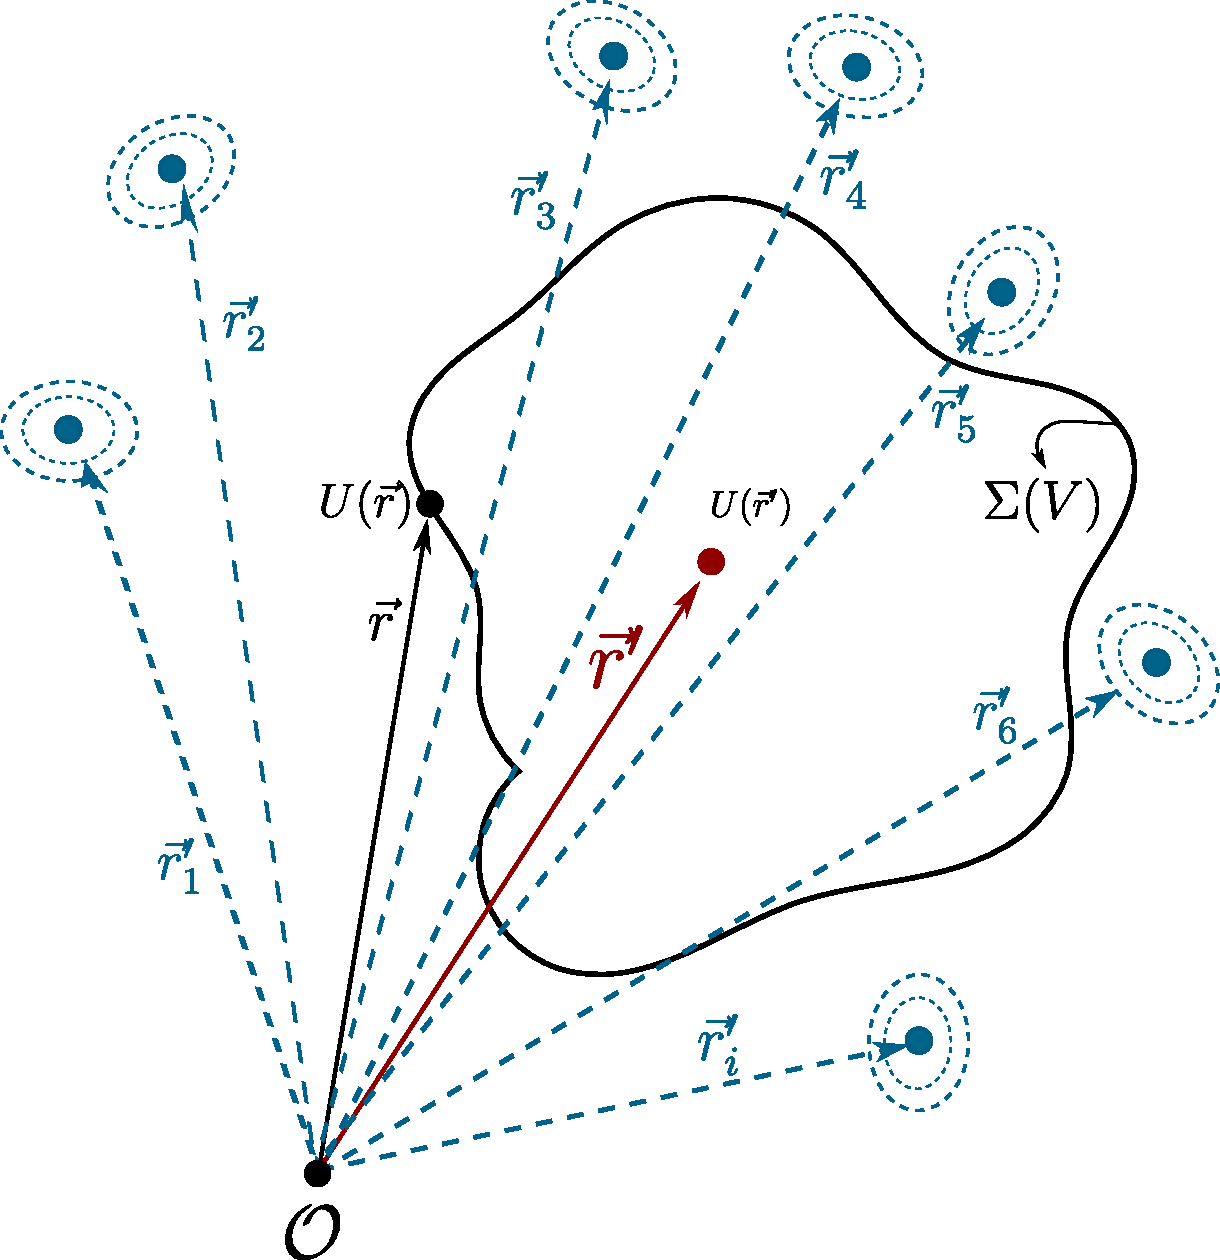
\includegraphics[width=0.7\linewidth]{Chapter 5/Figures/GreenImagenes}
			\caption{On the boundary $\Sigma(V)$ the contribution of the field components $U(\vec{r})$ is shown; inside the region the total field is built from the contribution of all the points on the boundary. One may add infinitely many point Green charges of arbitrary propagation nature; the condition for the invariance of equation \eqref{eq:GreenHomogeneous} is that these image charges lie outside $\Sigma(V)$.}
			\label{fig:greenimages}
		\end{figure}

		In this spirit, equation \eqref{eq:GreenHomogeneous} becomes

		\begin{equation}
			(\nabla^2 + k^2)G(\vec{r},\vec{r}') = 4\pi \delta(\vec{r}-\vec{r}') + 4\pi \sum_{i=1}^{\infty} \delta(\vec{r}-\vec{r}''_i).
		\end{equation}

		The explicit solution for a homogeneous medium of equation \eqref{eq:GreenHomogeneous} is

		\begin{equation}
			\label{sol_Green}
			G(\vec{r}, \vec{r}') = \frac{e^{ik\|\vec{r} - \vec{r}'\|}}{\|\vec{r} - \vec{r}'\|},
		\end{equation}

		corresponding to an outgoing spherical wave centred at $\vec{r}'$. Substituting $G$ into
		Green's identity, one derives

		\begin{equation}
			\label{green}
			U(\vec{r}', \nu) = \frac{1}{4\pi} \oint_{\Sigma(V)} \left[ U(\vec{r}, \nu)\nabla G(\vec{r}, \vec{r}')- G(\vec{r}, \vec{r}')\nabla U(\vec{r}, \nu)  \right ] \cdot d\vec{\sigma},
		\end{equation}

		known as the HelmholtzKirchhoff integral formula. This equation allows $U(\vec{r}',
		\nu)$ to be computed at any point of the volume $V$ by means of an integral over its
		boundary $\Sigma(V)$.

		\begin{figure}[htbp]
			\centering
			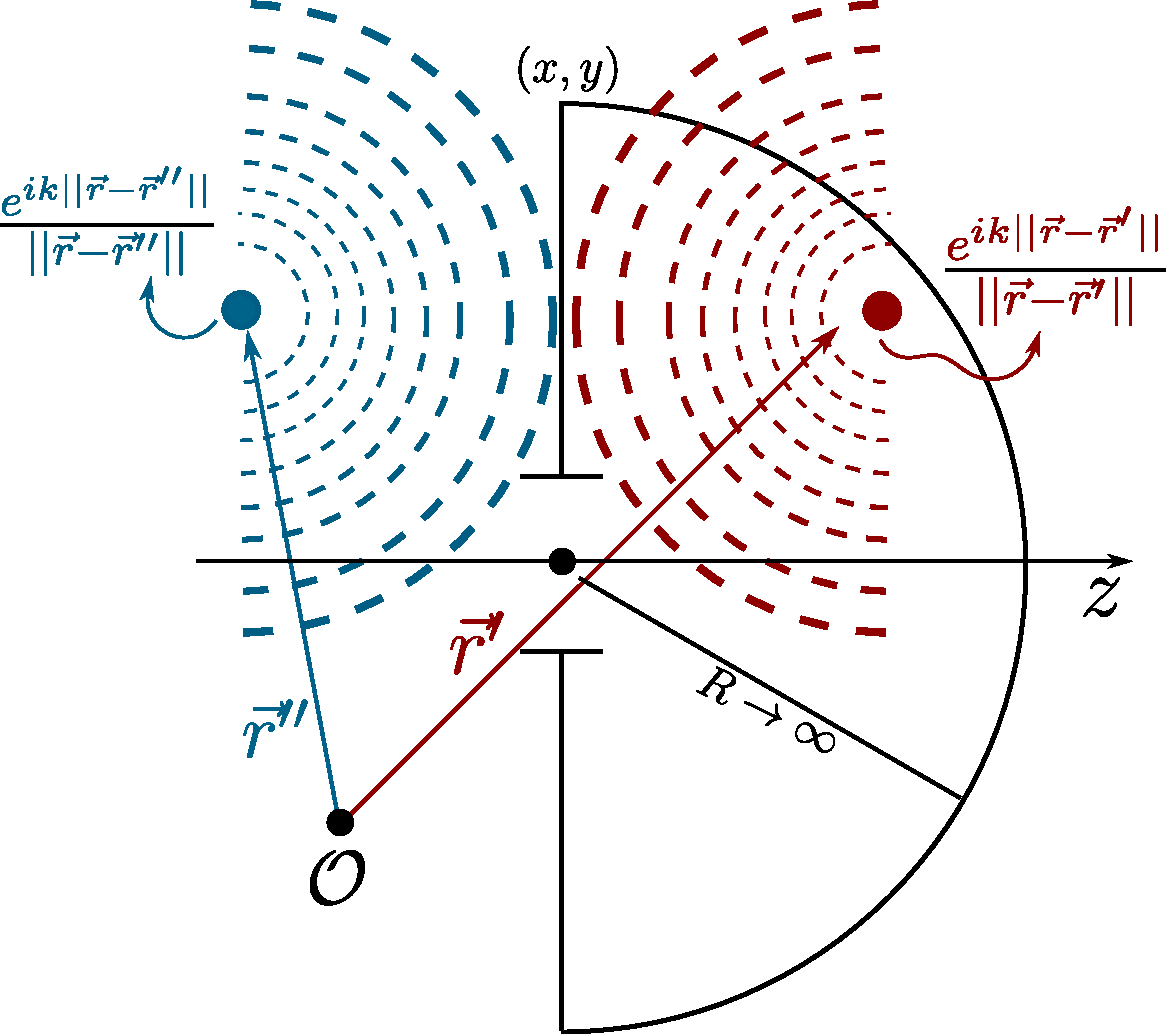
\includegraphics[width=0.7\linewidth]{Chapter 5/Figures/GreenPuntual}
			\caption{Representation of the Green's functions for point sources. Under these boundary conditions the Green's functions behave as point charges, one the mirror image of the other.}
			\label{fig:greenpoint}
		\end{figure}

		Before continuing, it is worth noting that the point-charge nature of the Green's functions
		$G(\vec{r},\vec{r}')$ is an assumption taken for granted; there is, however, no restriction
		on their physical nature. As is well known in electromagnetic theory, radiation sources may
		have any volume and shape, so our problem (Figure~\ref{fig:greenpoint}) can be made more
		general, as shown in Figure~\ref{fig:greennonpoint}, and the differential equation for
		Green's functions with volume would read

		\begin{equation}
			\left( \nabla^2 + k^2 \right)G(\vec{r},\vec{r}') = 4\pi \rho(\vec{r}-\vec{r}'_+) - 4\pi\rho(\vec{r}-\vec{r}'_-).
		\end{equation}

		\begin{figure}[htbp]
			\centering
			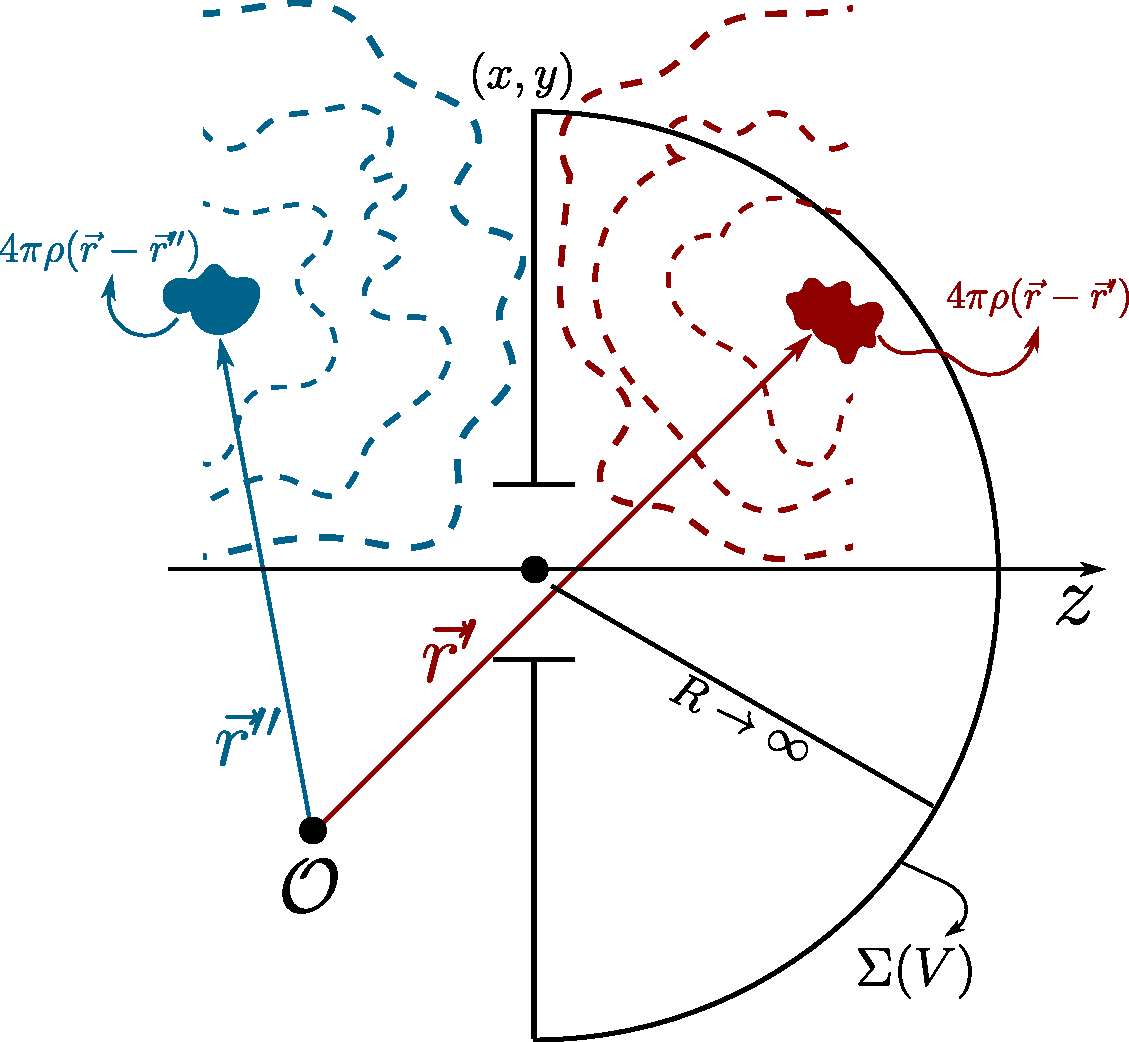
\includegraphics[width=0.7\linewidth]{Chapter 5/Figures/GreenNoPuntual}
			\caption{Representation of the Green's functions for non-point sources. Under these boundary conditions the Green's functions still behave as mirror images, but now with given volume and geometry; the only constraint on the emission of these sources is that, on the boundary $z=0$, the total field must vanish, as required by the assumed Dirichlet conditions.}
			\label{fig:greennonpoint}
		\end{figure}

		Let us continue with the development for point Green's functions. To simplify the
		evaluation of the integral, we consider a volume $V$ bounded by an infinite plane
		$\Sigma_1$ ($z=0$) and a hemisphere $\Sigma_2$ of radius $R$ (see
		Figure~\ref{fig:greenpoint}). The contribution of $\Sigma_2$ vanishes as $R \to \infty$
		(owing to the Sommerfeld radiation condition), reducing the expression to

		\begin{equation}
			U(\vec{r}', \nu) = \frac{1}{4\pi} \int_{\Sigma_1} \left[U(\vec{r}, \nu)\frac{\partial G}{\partial n} -   G(\vec{r}, \vec{r}')\frac{\partial U}{\partial n} \right] d\sigma,
		\end{equation}

		where $\frac{\partial}{\partial n} = \hat{n} \cdot \nabla$ denotes the normal derivative.
		However, this formulation requires specifying simultaneously $U$ and $\partial U/\partial
		n$ on $\Sigma_1$, which over-determines the problem. This difficulty motivates the
		introduction of physically realistic boundary conditions, such as those of Kirchhoff, in
		order to resolve the ambiguity.

		This problem is aggravated by a theorem of complex analysis, attributed to Riemann, which
		states that if a function and its normal derivative vanish on an open region of a plane,
		then the function must be identically zero throughout the domain. This restriction
		motivates the strategic need to eliminate one of the terms in the HelmholtzKirchhoff
		surface integral.

		The key is to exploit the degrees of freedom inherent in the choice of the auxiliary
		Green's function $G$. Kirchhoff initially proposed the intuitive boundary conditions
		\begin{itemize}
			\item $U = 0$ outside the aperture on $\Sigma$ (blocked field),
			\item $\partial U/\partial n = 0$ on opaque regions (vanishing normal derivative).
		\end{itemize}

		Although these conditions reproduced the experimental results of diffraction, they
		introduced mathematical inconsistencies by violating the CauchyRiemann uniqueness
		theorem. Poincaré showed that such assumptions generate contradictions in the mixed
		derivatives of the field. The resolution came with Sommerfeld, who redefined $G$ by means
		of a double-layer (mirror) Green's function, ensuring that
		\begin{itemize}
			\item $G = 0$ on $\Sigma$ (Dirichlet condition),
			\item $\partial G/\partial n$ remains non-singular,
		\end{itemize}

	thus eliminating the redundancy in the boundary conditions and preserving the
	self-consistency of the formalism.

	\subsection{The RayleighSommerfeld formulation}

		Returning to equation \eqref{green} and choosing the Dirichlet condition for the function
		$G$, we have

		\begin{equation}
			\label{psi_expr}
			U(\vec{r}', \nu) = \frac{1}{4\pi} \int_{\Sigma_1} \left[U(\vec{r}, \nu) \nabla G \cdot\hat{n}\right] d\sigma .
		\end{equation}

		Given the integration surface under consideration, we may express \eqref{sol_Green} as

		\begin{equation}
			\label{sol_Green_RS}
			G(\vec{r}, \vec{r}') = \frac{e^{ik\|\vec{r} - \vec{r}'\|}}{\|\vec{r} - \vec{r}'\|} - \frac{e^{ik\|\vec{r} - \vec{r}''\|}}{\|\vec{r} - \vec{r}''\|},
		\end{equation}

		\noindent where
		\begin{align}
			\|\vec{r} - \vec{r}''\| &= \|\vec{r} - \vec{r}'\|, \qquad x'' = x', \quad y'' = y', \quad z'' = -z',
		\end{align}

		since $\vec{r}''$ is the mirror image of $\vec{r}'$ across the plane $\Sigma_1$. It follows
		that

		\begin{equation}
			\nabla G \cdot \hat{z}  = 2 \left[ik - \dfrac{1}{\|\vec{r}-\vec{r}'\|} \right]\dfrac{e^{ik\|\vec{r}-\vec{r}'\|}}{\|\vec{r}-\vec{r}'\|} \cos(\vec{r} - \vec{r}',\hat{z}),
		\end{equation}

		and with this, \eqref{psi_expr} becomes

		\begin{equation}
			U(\vec{r}',\nu) = \dfrac{1}{2\pi} \int_{\Sigma} U(\vec{r},\nu) \left[ik - \dfrac{1}{\|\vec{r} - \vec{r}'\|} \right] \dfrac{e^{ik\|\vec{r}-\vec{r}'\|}}{\|\vec{r}-\vec{r}'\|} \cos(\vec{r} - \vec{r}',\hat{z})\,d\sigma .
		\end{equation}

		We may now make the approximation appropriate to the RayleighSommerfeld regime, in which
		$\|\vec{r}-\vec{r}'\| \gg \lambda$, obtaining

		\begin{equation}
			U(\vec{r}',\nu) = \dfrac{ik}{2\pi} \int_{\Sigma} U(\vec{r},\nu)\dfrac{e^{ik\|\vec{r}-\vec{r}'\|}}{\|\vec{r}-\vec{r}'\|} \cos(\vec{r} - \vec{r}',\hat{z})\,d\sigma,
		\end{equation}

		a mathematical expression that embodies the HuygensFresnel principle: as can be
		appreciated, there is one spherical wave per point of the integration surface.

\section{The Fresnel approximation}

Starting from the field

\begin{align}
	U(\vec{r}') = \frac{ik}{2\pi}\int_{\Sigma} U(\vec{r}) \frac{e^{ik \left\| \vec{r} - \vec{r}' \right\|}}{\left\| \vec{r} - \vec{r}' \right\|} \cos(\vec{r} - \vec{r}', \hat{z}) \, \mathrm{d}\sigma,
\end{align}

it is possible to carry out the so-called mid-field or Fresnel approximation. To this end
we take

\begin{align}
	\label{aprox_r}
	\|\vec{r}-\vec{r}'\| &= \left[(x-x')^2 + (y-y')^2 + (z-z')^2\right]^{1/2} \notag \\
	&= z\left(1 + \dfrac{(x-x')^2 + (y-y')^2}{z^2} \right)^{1/2} \notag \\
	&\approx z + \dfrac{(x-x')^2+(y-y')^2}{2z}.
\end{align}

It is clear that, for the factor $\dfrac{1}{\|\vec{r}- \vec{r}'\|}$, an expansion up to the
first term of \eqref{aprox_r} suffices; this is not enough for the factor $e^{ik
\left\| \vec{r} - \vec{r}' \right\|}$, however, since the latter has oscillatory behaviour
over its domain, so both terms are required. We additionally take $\cos (\vec{r}-\vec{r}',
\hat{z}) = \dfrac{z}{\|\vec{r} - \vec{r} '\|} \approx 1$.

In this spirit, we obtain an expression for the field of the form

\begin{equation}
	\label{Fresnel}
	U(\vec{r}') = \dfrac{i e^{ikz}}{\lambda z} \int U(\vec{r}) \exp \left(\dfrac{ik}{2z} ((x-x')^2 + (y-y')^2) \right) d\sigma,
\end{equation}

which describes the propagation or diffraction of the electromagnetic field in the Fresnel
regime. It is worth stressing that equation \eqref{Fresnel} describes a parabolic wave,
and although, at least conceptually, such propagation is valid for a mid-field, in
practice it has proved more than sufficient for sufficiently short distances.

\section{The Fraunhofer approximation}

Finally, from expression \eqref{Fresnel} a second approximation may be carried out,
corresponding to the far field or Fraunhofer regime, in which the observation distances are
considerably larger than the area over which one wishes to study the propagated field
(whether through a slit or another object). We focus on the factor

\begin{align}
	\exp\left( \frac{ik}{2z} ((x-x')^2 + (y-y')^2) \right)
	&= \exp\left( \frac{ik}{2z} (x^2 + y^2) \right)
	\exp\left( \frac{ik}{2z} (x'^2 + y'^2) \right)
	\exp\left( -\frac{ik}{z} (xx' + yy') \right),
\end{align}

where we may make the far-field assumption $\exp\left( \frac{ik}{2z} (x^2 + y^2) \right)
\approx 1$, so that we obtain

\begin{equation}
	\label{Fraunhofer}
	U(\vec{r}') = \dfrac{e^{ikz}}{\lambda z} \exp \left(\dfrac{ik}{2z} (x'^2 + y'^2)\right) \int U(\vec{r}) \exp\left( -\frac{ik}{z} (xx' + yy') \right) d\sigma .
\end{equation}

There we can still appreciate a quadratic phase term outside the integral, usually called
the curvature factor, which shows precisely the dephasing induced by the difference of
optical path between a plane called the observation screen and a spherical surface of
radius $z$ (the propagation distance of the field along the optical axis) known as the
cardinal sphere. The introduction of this spherical surface is rather useful when one
wishes to describe Fraunhofer diffraction on a screen as a Fresnel propagation through two
confocal cardinal spheres, as shown in Figure~\ref{fig:cardinals}.

\begin{figure}[htbp]
	\centering
	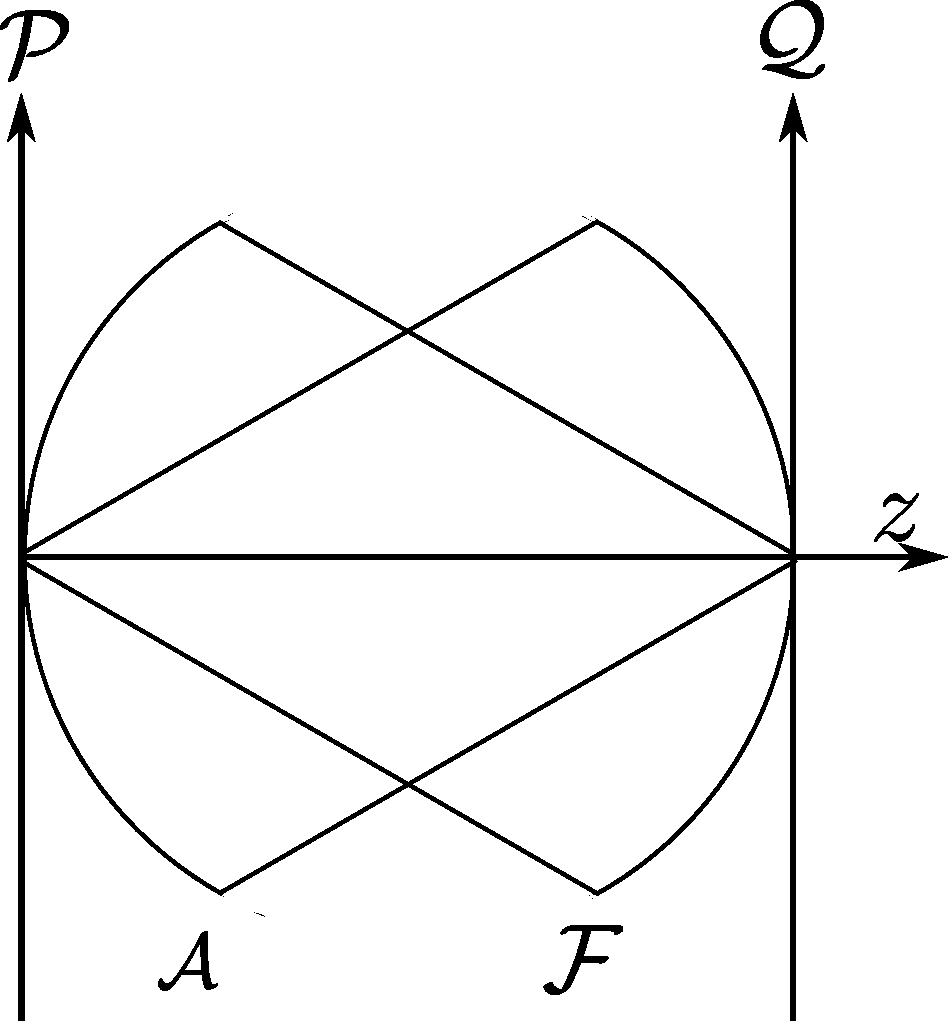
\includegraphics[width=0.5\linewidth]{Chapter 5/Figures/Cardinales}
	\caption{Scheme of the confocal cardinal spheres, with radii equal to the propagation distance $z$ of the field.}
	\label{fig:cardinals}
\end{figure}

This makes more sense once we analyse the effect of each propagation step. It is clear
that, without imposing far-field approximations from the outset, propagating the field at
$\mathcal{A}$ towards $\mathcal{F}$ with the Fresnel approximation, we would obtain

\begin{equation}
	U_{\mathcal{F}}(\vec{r}) = \dfrac{ie^{ikz}}{\lambda z} \exp\left( \frac{ik}{2z} (x^2 + y^2) \right)  \int u_{\mathcal{A}}
	\exp\left( \frac{ik}{2z} (x'^2 + y'^2) \right)
	\exp\left( -\frac{ik}{z} (xx' + yy') \right)d\sigma' ,
\end{equation}

where we may associate $u_{\mathcal{A}}$, i.e.\ the field on the sphere $\mathcal{A}$, with
the field on $\mathcal{P}$ multiplied by its corresponding quadratic factor
$u_{\mathcal{P}} = u_{\mathcal{A}} (\vec{r}') \exp{\left( \dfrac{ik}{2z}(x'^2+y'^2)
\right)}$, while the term $\exp{\left( \frac{ik}{2z} (x^2 + y^2) \right)}$ may be
understood as the factor resulting from passing the field from the sphere $\mathcal{F}$ to
the screen $\mathcal{Q}$, so that the field on $\mathcal{F}$ would correspond to

\begin{equation}
	u_{\mathcal{Q}}(\vec{r}) = \dfrac{ie^{ikz}}{\lambda z} \int u_{\mathcal{P}}
	\exp\left( -\frac{ik}{z} (xx' + yy') \right)d\sigma' ,
\end{equation}

thus recovering a Fraunhofer expression for diffraction on $\mathcal{Q}$. It should be
noted that one must check whether the study of the propagated field is valid within a
paraxial regime, where the field is confined to the neighbourhood of the optical axis and
hence the curvature of the cardinal sphere does not differ much from the plane (the
screen). In cases where the curvature factor ceases to be negligible, the paraxial regime
loses validity and the problem must be addressed from a meta-axial standpoint.

Studying the propagation of the field through Fresnel diffraction is of great importance
because, as will be discussed later, it bears a close relationship with what is known as
the fractional Fourier transform, a tool that arises naturally when one chains paraxial
propagation steps.
